% !TeX program = xelatex
\documentclass[UTF8,fontset=fandol,10pt,a4paper]{ctexart}
\usepackage[left=22mm,right=22mm,top=23mm,bottom=22mm,headheight=14pt]{geometry}
\usepackage{fontspec}
\setmainfont{TeX Gyre Heros}
\setsansfont{TeX Gyre Heros}
\setmonofont{Latin Modern Mono}
\renewcommand{\familydefault}{\sfdefault}
\usepackage[table]{xcolor}
\usepackage{graphicx,tikz}
\usetikzlibrary{arrows.meta,positioning,fit,backgrounds,calc}
\usepackage{booktabs,tabularx,array,enumitem,float,caption,fancyhdr,hyperref}
\definecolor{blue}{HTML}{2869A9}
\definecolor{ink}{HTML}{293340}
\definecolor{muted}{HTML}{647181}
\definecolor{line}{HTML}{C5D4E2}
\definecolor{pale}{HTML}{F0F5FA}
\definecolor{warm}{HTML}{FFF7E9}
\hypersetup{colorlinks=true,urlcolor=blue,linkcolor=blue,pdftitle={Redflag RHI 与 Vulkan 接入设计},pdfauthor={Redflag}}
\color{ink}
\setlength{\parindent}{0pt}
\setlength{\parskip}{6pt}
\linespread{1.16}
\setlist[itemize]{leftmargin=1.5em,itemsep=2pt,topsep=3pt}
\setlist[enumerate]{leftmargin=1.8em,itemsep=3pt,topsep=3pt}
\renewcommand{\arraystretch}{1.38}
\newcolumntype{Y}{>{\raggedright\arraybackslash}X}
\newcolumntype{L}[1]{>{\raggedright\arraybackslash}p{#1}}
\ctexset{section={format=\Large\bfseries\color{blue},beforeskip=16pt,afterskip=8pt},subsection={format=\large\bfseries\color{blue},beforeskip=11pt,afterskip=5pt}}
\captionsetup{font=small,labelfont=bf,textfont={color=muted},skip=7pt}
\pagestyle{fancy}\fancyhf{}
\fancyhead[L]{\small\color{muted}Redflag · RHI / Vulkan · 设计方案}
\fancyhead[R]{\small\color{muted}2026-11-21}
\fancyfoot[C]{\small\color{muted}\thepage}
\renewcommand{\headrulewidth}{0pt}
\newcommand{\note}[1]{{\small\color{muted}#1\par}}
\newcommand{\code}[1]{{\small\texttt{#1}}}
\newcommand{\ruleline}{\par\vspace{4pt}{\color{line}\hrule}\vspace{8pt}}
\newcommand{\source}[2]{{\small\href{#1}{[#2]}}}
\tikzset{
 module/.style={draw=line,fill=pale,rounded corners=2pt,align=center,inner sep=7pt,text width=3.8cm,minimum height=1.15cm,font=\small},
 smallbox/.style={module,text width=2.55cm,minimum height=.95cm,font=\footnotesize},
 wide/.style={module,text width=9.5cm},
 planned/.style={module,fill=warm,dashed},
 flow/.style={-{Stealth[length=2mm]},draw=muted,line width=.65pt},
 own/.style={flow,dashed},
 label/.style={font=\scriptsize,fill=white,inner sep=2pt,text=muted}}

% 本册的页幅、图注和代码排版。
\geometry{paperwidth=190mm,paperheight=252mm,left=21mm,right=21mm,
  top=22mm,bottom=21mm,headheight=21pt,headsep=4mm,footskip=10mm}
\usepackage{amsmath,listings,type1cm}
\definecolor{Ink}{HTML}{202E33}
\definecolor{Muted}{HTML}{4C6064}
\definecolor{Teal}{HTML}{12665F}
\definecolor{Rust}{HTML}{9E452B}
\definecolor{Rule}{HTML}{B3C6C1}
\definecolor{Soft}{HTML}{EAF3F0}
\definecolor{Paper}{HTML}{FFFFFF}
\setmainfont{TeX Gyre Pagella}
\renewcommand{\familydefault}{\rmdefault}
\linespread{1}
\setcounter{secnumdepth}{0}
\setlength{\emergencystretch}{2em}
\setlength{\parindent}{0pt}
\setlength{\parskip}{5.8pt}
\ctexset{section={format=\raggedright\sffamily\bfseries\fontsize{23}{30}\selectfont\color{Ink},
    beforeskip=0pt,afterskip=9pt},
  subsection={format=\raggedright\sffamily\bfseries\fontsize{13}{18}\selectfont\color{Teal},
    beforeskip=8pt,afterskip=2pt}}
\hypersetup{urlcolor=Teal,linkcolor=Teal,bookmarksnumbered=false,
  pdfsubject={Redflag 渲染接口、后端实现与验证}}
\fancyhf{}
\setlength{\headwidth}{\textwidth}
\fancyhead[L]{\sffamily\fontsize{9.5}{12}\selectfont\bfseries\color{Teal}Redflag\enspace{\mdseries\color{Muted}图形引擎}}
\fancyhead[R]{\sffamily\small\color{Muted}RHI / Vulkan}
\renewcommand{\headrule}{\hbox to\headwidth{\color{Rule}\leaders\hrule height .55pt\hfill}}
\fancyfoot[L]{\small\sffamily\color{Muted}\nouppercase{\leftmark}}
\renewcommand{\sectionmark}[1]{\markboth{#1}{}}
\fancyfoot[R]{\large\sffamily\bfseries\color{Teal}\thepage}
\renewcommand{\code}[1]{{\ttfamily\fontsize{10.4}{14}\selectfont #1}}
\newcommand{\readings}[1]{\par\noindent{\sffamily\fontsize{9.6}{14}\selectfont
  \color{Muted}参考\enspace #1\par}}
\newcommand{\refitem}[2]{\href{#1}{#2}}
\newcommand{\figpanel}[2]{\begin{figure}[H]\centering\input{figures/#1}\caption{#2}\end{figure}}
\DeclareCaptionFont{rhicapt}{\sffamily\fontsize{10}{14}\selectfont\color{Muted}}
\captionsetup{font=rhicapt,labelfont={bf,color=Teal},textfont=rhicapt,
  labelsep=quad,justification=raggedright,singlelinecheck=false,skip=4pt}
\setlength{\intextsep}{7pt plus 1pt minus 1pt}
\lstset{basicstyle=\ttfamily\fontsize{10.7}{15}\selectfont\color{Ink},
  backgroundcolor=\color{Soft},frame=l,rulecolor=\color{Teal},framerule=1.5pt,
  xleftmargin=5mm,xrightmargin=2mm,framexleftmargin=3mm,framesep=2pt,
  aboveskip=6pt,belowskip=6pt,columns=fullflexible,keepspaces=true,showstringspaces=false}
\newcommand{\bodytype}{\normalfont\fontsize{11.4}{17.8}\selectfont\color{Ink}}

\geometry{paperwidth=196mm,paperheight=264mm,left=19mm,right=19mm,top=21mm,bottom=21mm}
\hypersetup{pdftitle={RedflagForge 编辑器入门},pdfauthor={Redflag},pdfsubject={场景、摄像机、实时效果和保存}}
\fancyhead[L]{\sffamily\small\bfseries\color{Teal}RedflagForge}
\fancyhead[R]{\sffamily\small\color{Muted}编辑器入门\enspace / \enspace Vulkan}
\setlength{\parindent}{2\ccwd}
\setlength{\parskip}{5pt}
\ctexset{section={afterindent=true},subsection={afterindent=true}}
\graphicspath{{figures/}{../../../output/rhi/}}
\newcommand{\ui}[1]{{\sffamily\bfseries\color{Teal}#1}}
\newcommand{\tabhead}[1]{{\sffamily\bfseries\color{Teal}#1}}
\newcommand{\numtag}[1]{\tikz[baseline=(tag.base)]{\node[shape=circle,inner sep=0pt,minimum size=4.7mm,fill=Teal,text=white,font=\sffamily\bfseries\footnotesize](tag){#1};}}
\newcommand{\captionline}[1]{\par\noindent{\sffamily\fontsize{9.6}{14}\selectfont\color{Muted}#1\par}}
\newcommand{\shots}[2]{\begin{minipage}[t]{.484\linewidth}\includegraphics[width=\linewidth]{#1}\captionline{#2}\end{minipage}}
\newcommand{\tabletype}{\small\sffamily\renewcommand{\arraystretch}{1.45}}
\newcommand{\toolbar}{实时效果}
\begin{document}
\bodytype
\section{RedflagForge 编辑器入门}
打开编辑器，首先看见的是 Sponza 中庭。走廊里的布帘、地砖和廊柱属于同一个模型。场景中另有三盏可以单独移动的灯。调灯时让镜头停在原处，地面上哪里变亮、柱子在哪一侧投下阴影，就容易看清了。

\begin{figure}[H]\centering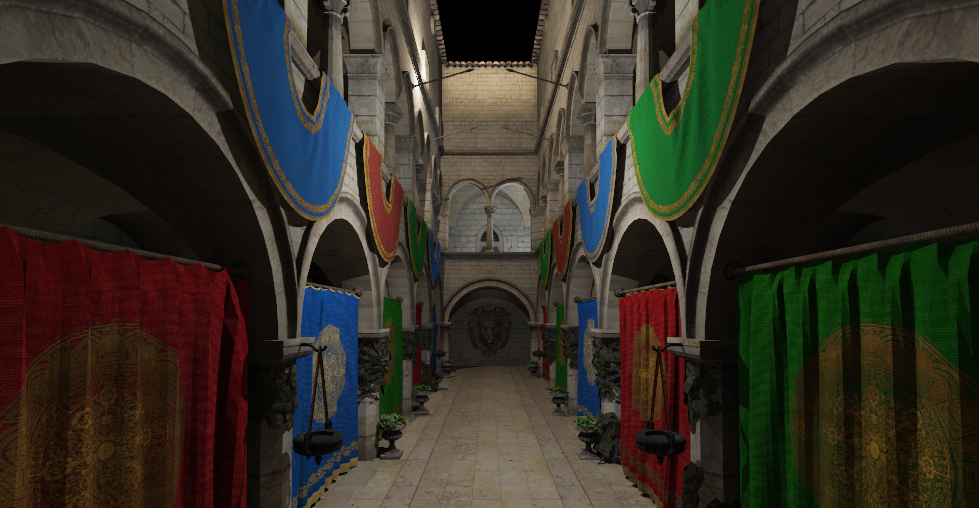
\includegraphics[width=\linewidth]{atrium.png}
\caption{Vulkan 编辑器中的 Sponza 中庭。为方便对照材质、墙角和灯光，此图截取自实际场景视口。}
\end{figure}

如果已有 Debug/x64 构建和 Sponza 模型，双击仓库根目录的 \path{Open-Vulkan-Editor.cmd} 即可进入中庭。第一次从源码运行时，用 Visual Studio 打开 \path{Redflag.sln}，选择 \ui{Debug / x64}，生成 \ui{RedflagForge} 项目。源码构建需要 Visual Studio 的 C++ 工具链和 Vulkan SDK。

如果还缺少中庭模型，在仓库根目录的 PowerShell 运行第一条命令，下载 glTF 网格和配套贴图。下载完成后运行第二条命令，打开编辑器。
\begin{lstlisting}[basicstyle=\ttfamily\fontsize{9.6}{13.5}\selectfont]
# 仓库根目录。先准备场景资源，再启动 Vulkan 编辑器。
python tests/fetch_sponza.py
.\Open-Vulkan-Editor.cmd
\end{lstlisting}
进入后在菜单栏可以看到场景名 \ui{Sponza-Atrium}。若已在其他场景，从“文件 → 打开场景…”选中 \path{assets/scenes/Sponza-Atrium.redflag}。脚本会传入 \code{--vulkan}。直接运行可执行文件且未加此参数时，程序使用 OpenGL。

\clearpage
\section{场景、相机与点光源}
\begin{figure}[H]\centering
\begin{tikzpicture}
  \node[inner sep=0,anchor=south west] (photo) at (0,0) {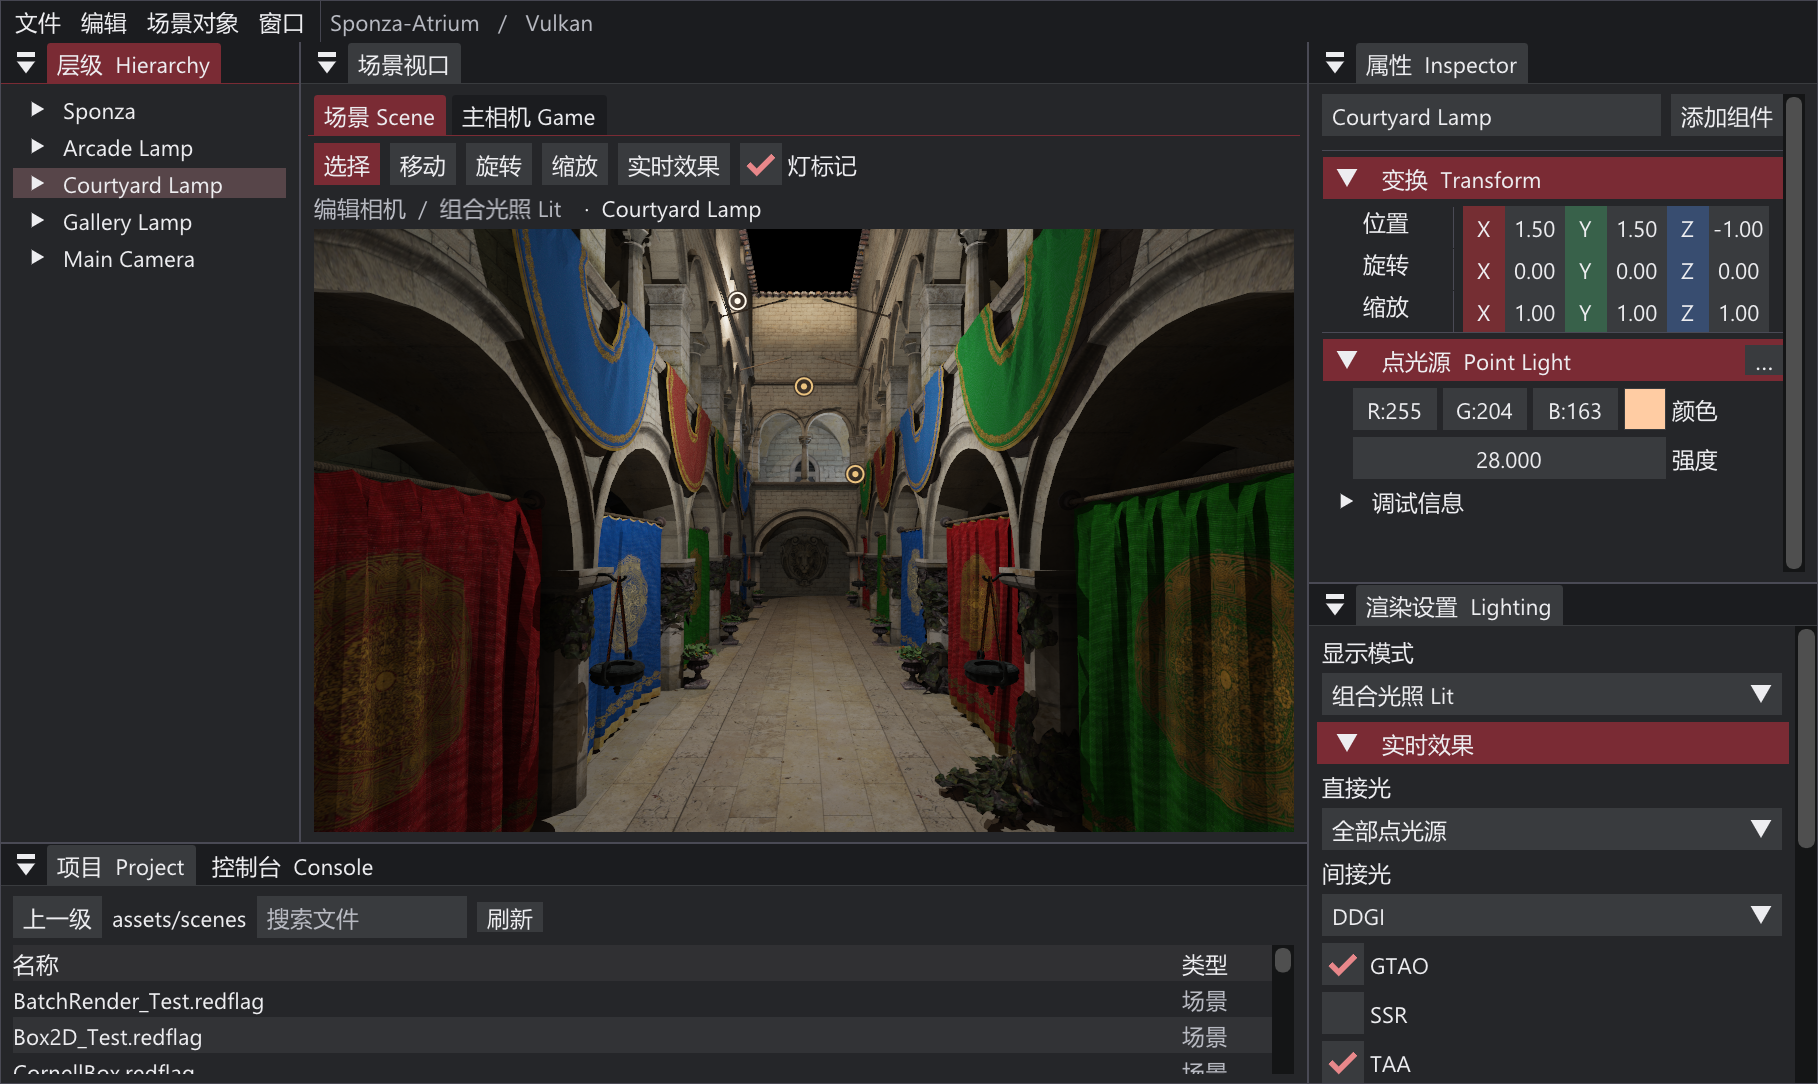
\includegraphics[width=\linewidth]{editor-light-inspector.png}};
  \begin{scope}[x={(photo.south east)},y={(photo.north west)}]
    \tikzset{marker/.style={circle,draw=white,line width=.8pt,fill=Teal,text=white,
      minimum size=5.6mm,inner sep=0pt,font=\sffamily\bfseries\small}}
    \node[marker] at (.135,.83) {1};
    \node[marker] at (.960,.583) {2};
    \node[marker] at (.688,.62) {3};
    \node[marker] at (.644,.16) {4};
  \end{scope}
\end{tikzpicture}
\caption{实际编辑器全窗。按编号可找到层级、属性、场景视口和项目文件。面板停靠位置可调整，本页使用默认布局。}
\end{figure}


找物体看左边的“层级”，改它的属性看右边的“属性”，要改变画面则看视口上方的“实时效果”。图中 \numtag{1}\,列出了当前场景的物体。点击 \ui{Courtyard Lamp}，\numtag{2}\,的属性随之切换到这盏灯。在“点光源 Point Light”中把“强度”从场景预设的 28 降到 8，观察中庭灯光的亮度，再将它调回 28。也可以在场景视口点“移动”（W），拖动彩色轴箭头，灯和亮斑会跟着移动。查看效果时先在渲染设置选“组合光照 Lit”，直接光选“全部点光源”。

\numtag{3}\,是画面所在的视口。\ui{场景 Scene}使用编辑器相机。鼠标放进画面，按住左 Alt 拖动左键可绕观察中心旋转，左 Alt 加中键平移，滚轮拉近或拉远。普通左键点击可选中模型或灯的圆形标记，点击背景会清空选择。Sponza 整座建筑是一个实体，想调整一盏灯时从列表选择最方便。

\ui{主相机 Game}使用场景的主相机。切到这个标签，可以在保持镜头不动的情况下调灯、比较效果。想换机位时，回到场景标签自由观察。要改变游戏画面的机位，则在实体列表选中 \ui{Main Camera}，编辑它的变换。

\numtag{4}\,是项目文件。首次打开会列出 \path{assets/scenes}，在此双击某个 \path{.redflag} 文件即可切换场景。要试一个单独的雕塑，从仓库根目录先运行 \code{python tests/fetch\_stanford.py}，再打开 \path{Reference-StanfordBunny.redflag}。每次换场景前可先保存自己的修改。

\clearpage
\section{开启实时效果}
固定在\ui{主相机 Game}机位，点击视口上的\ui{\toolbar}。弹层中可以选择直接光和间接光的算法，也可以勾选 GTAO、SSR、镜面 IBL、体积雾和 TAA。改动这里的效果会切换到\ui{组合光照 Lit}，在同一幅画面上看到它们的结果。

\begin{figure}[H]\centering
\begin{minipage}[c]{.495\linewidth}
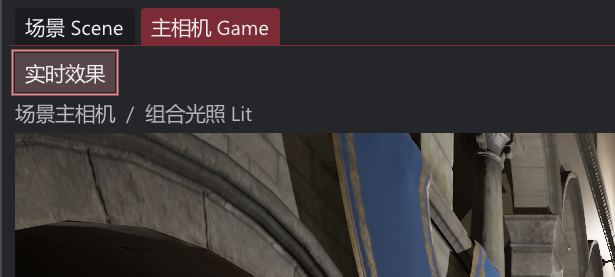
\includegraphics[width=\linewidth]{effects-button.png}
\captionline{\numtag{1}\enspace 在场景视口的工具栏点击“实时效果”。}
\end{minipage}\hfill
\begin{minipage}[c]{.44\linewidth}\centering
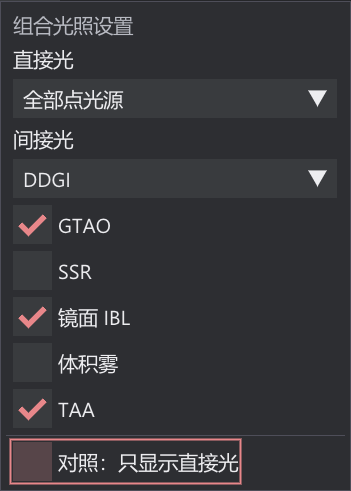
\includegraphics[height=80mm]{effects-menu.png}
\captionline{\numtag{2}\enspace 选择光照方法，勾选要叠加的效果。}
\end{minipage}
\caption{Sponza 中庭的主相机视图。图中选用全部点光源和 DDGI，已勾选 GTAO、镜面 IBL 和 TAA。SSR 与体积雾的方框为空，点击方框即可启用。}
\end{figure}


把“直接光”设为\ui{全部点光源}，让场景里的每一盏灯都参与计算。“间接光”先选\ui{关闭}，看廊柱背面和拱廊内侧。再选\ui{DDGI}，停一下让反射光逐帧积累。若只想比较完整设置和直接光，可勾选\ui{对照：只显示直接光}，再取消勾选即可返回。

有了间接光，可以勾选\ui{GTAO}。看柱脚与地面的交界，附近表面挡住一部分反射光，交界处会变暗。关闭间接光时，此项变灰。勾选\ui{SSR}后可观察地面上的反射。沿地面寻找另一块表面时，只能找到当前镜头内已有的信息。

打开\ui{TAA}，保持相机不动，观察远处细栏杆和布帘边缘。它会合并几个取样位置的颜色，需等待数帧。要在同一帧内多取几个位置，可试第\pageref{sec:ssaa}页的\ui{SSAA 2×2}。想单看某道效果，使用渲染设置中的\ui{显示模式}。返回\ui{组合光照 Lit}可继续看几种效果共同作用的画面。

\clearpage
\section{固定机位比较画面}
\begin{figure}[H]\centering
\shots{before.png}{间接光关闭}\hfill
\shots{after.png}{开启探针间接光 DDGI}
\caption{均为 Sponza 主相机视口的同一处裁图。看红布幔上方的拱廊内侧，左图几乎全黑，右图能分清拱顶与侧墙。两次都用全部点光源，SSR 关闭，TAA 开启。GTAO 保持勾选，只有右图有间接光可供它衰减。}
\end{figure}


切到\ui{主相机 Game}，将分辨率设为\ui{原始 Native}，选定一个物体作为观察位置。要看间接光，保留直接光和其他效果的设置，只改变间接光。要看环境遮蔽，保留同一种间接光，只开关 GTAO。这样可以分清阴影来自灯被挡住，还是周围表面遮住了反射光。

{\noindent\tabletype\begin{tabularx}{\linewidth}{@{}p{30mm}X@{}}\toprule
\tabhead{想比较什么}&\tabhead{在哪儿看、怎样调整}\\\midrule
直接光采样 & “全部点光源”逐盏计算，可当作本场景的直接光参照。ReSTIR DI 重用附近像素或上一帧挑中的灯。比较时留意帘幕边缘和柱子的阴影。\\
墙面的反光 & 选择 DDGI，勾选“多次漫反射”后，到达一面墙的反光还能照到邻近表面。来回切换，比较柱脚和拱廊内侧的亮度。\\
反射细节 & 在“显示模式”选 SSR，展开“质量与参数”，拖动“示例粗糙度”观察倒影的轮廓。切回“组合光照 Lit”并勾选 SSR，地板和柱子各用自己的材质粗糙度。有贴图时，绿色通道的值还要乘上材质的粗糙度系数。\\
\bottomrule\end{tabularx}\par}

组合光照（Lit）默认在移动镜头时保留间接光和已开启的效果。勾选\ui{移动时仅算直接光}再拖动相机，可以单独看灯直接照亮的部分，停手后会恢复完整光照。

镜头停下后，只算普通直接光，一帧就够了。打开 TAA，同一条边会在后续几帧从略微不同的位置取样，再合成较平滑的轮廓。ReSTIR DI 也会沿用前几帧选中的灯。这些效果开启时，镜头不动，编辑器最多连续画 32 帧。32 是项目试用后选的帧数。画完后，面板继续显示最后一张图，直到再次移动镜头或调整灯光。

\clearpage
\section{保存与恢复}
选择“文件 → 另存为…”，把示例另存为 \path{MyAtrium.redflag}。\ui{Ctrl + Shift + S} 选择保存位置并写入副本，之后用 \ui{Ctrl + S} 将改动写回这个副本。保存会生成两份相邻的文件。重新打开时，选择扩展名为 \path{.redflag} 的那一个。

{\noindent\tabletype\begin{tabularx}{\linewidth}{@{}p{57mm}X@{}}\toprule
\tabhead{文件}&\tabhead{重新打开时用到的数据}\\\midrule
\path{MyAtrium.redflag} & 场景中的实体、模型引用、变换、相机和点光源。\\
\path{MyAtrium.redflag.render.yaml} & 显示模式、直接光与间接光选项、效果开关、预览宽度和质量设置。\\
\bottomrule\end{tabularx}\par}

想重新熟悉面板位置，打开窗口菜单，选择“恢复默认布局”。如果想重看灯光刚开启时的样子，在渲染设置展开“质量与参数”，点“重新积累”。灯和效果设置保留下来，画面从第一帧开始逐渐稳定。

能看到实体名却看不到中庭时，先看控制台最近一条提示。模型文件可由第 1 页的下载命令补齐，然后重新打开 Sponza 场景。新建场景默认以材质底色显示，要试灯光，先从“场景对象”菜单分别创建“立方体”和“点光源”，在属性里把点光源放到立方体前上方，再按第 3 页的方法打开组合光照。

\begin{figure}[H]\centering
\begin{minipage}[c]{.49\linewidth}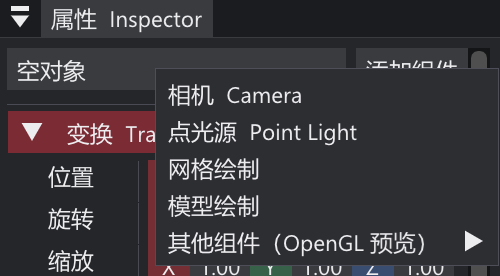
\includegraphics[width=\linewidth]{add-component.png}\end{minipage}\hfill
\begin{minipage}[c]{.46\linewidth}\caption{也可以让一个已有的空对象发光。选中它，在右侧属性点“添加组件”，再选“点光源 Point Light”。随后这里会出现颜色和强度。}\end{minipage}
\end{figure}

主相机标签提示没有主相机时，从“场景对象”菜单添加相机。没有主相机的场景会把新加的这台设为主相机。若误改了练习副本，可以重新打开保留的示例。若希望保留刚刚调好的灯光，请先保存副本。

想知道为什么柱脚会变暗，读《实时光照与采样》的环境遮蔽章节。想看同一机位开关效果的误差、耗时和原始截帧，读《渲染性能实测》的 Sponza 部分。想进一步看打开场景时有哪些类参与，可从《源码导读》读起。相关 PDF 位于项目的 \path{output/pdf/} 目录。

\clearpage
\section{保存房间里的反射光}
在仓库根目录运行 \code{python tests/fetch\_rtxgi\_bathroom.py}，打开 \path{assets/scenes/RTXGI-Bathroom.redflag}。选择\ui{组合光照 Lit}，将“间接光”设为\ui{DDGI}。在\ui{质量与参数}中可以看到\ui{DDGI 探针：已烘焙}，表示房间已读入上次保存的反射光。

\begin{figure}[H]\centering
\begin{minipage}[c]{.53\linewidth}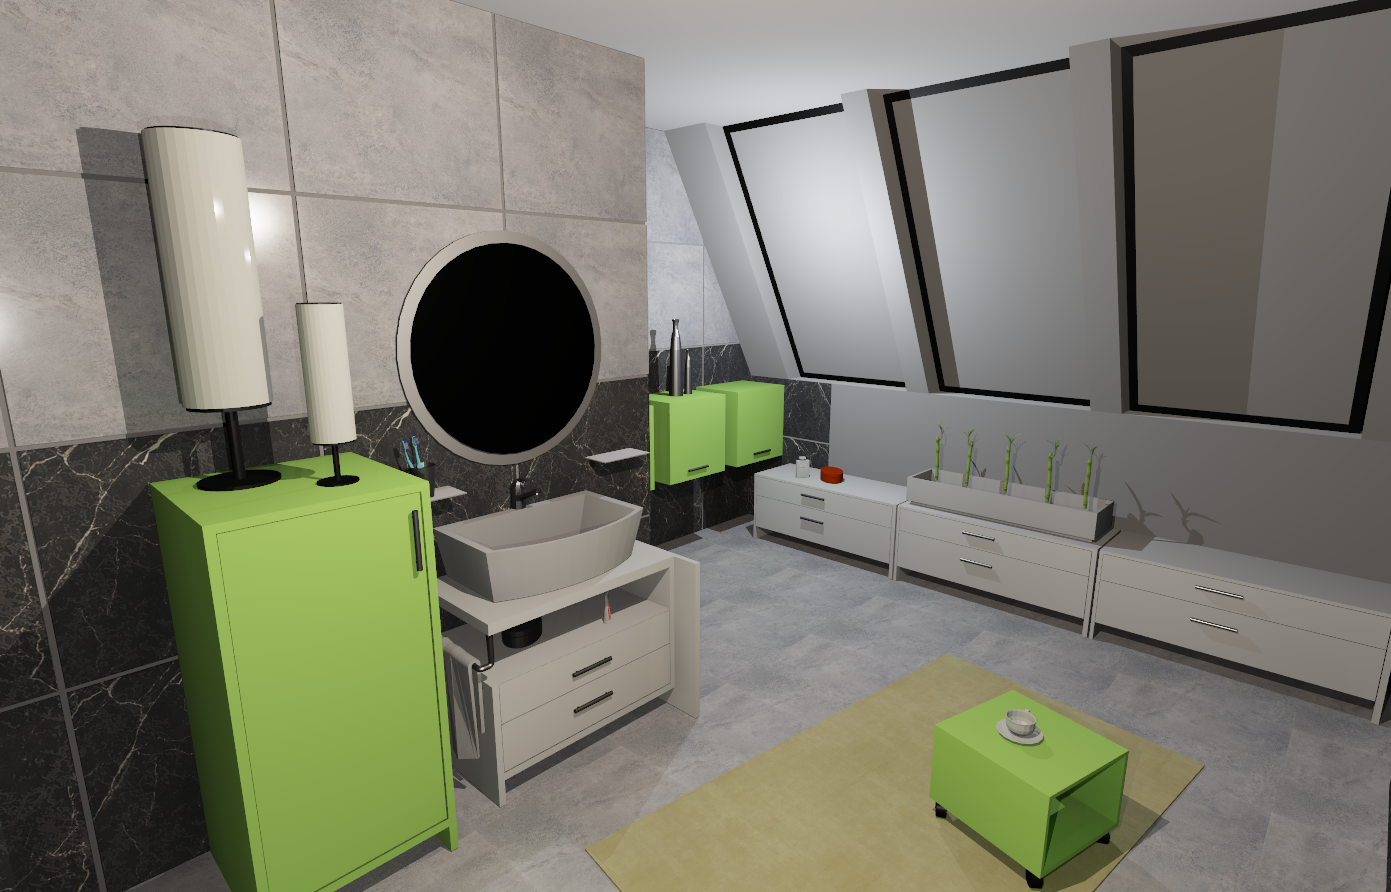
\includegraphics[width=\linewidth]{../../../output/profiling/point-materials/bathroom-pbr.png}\end{minipage}\hspace{.04\linewidth}
\begin{minipage}[c]{.32\linewidth}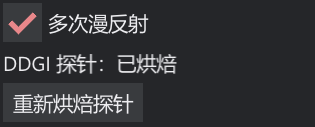
\includegraphics[width=\linewidth]{../../../output/profiling/point-materials/bathroom-reopened.png}\end{minipage}
\caption{重新打开 NVIDIA RTXGI 浴室。右图显示已开启多次漫反射，也已读入烘焙文件。}
\end{figure}

先用\ui{另存为}建一个练习副本，移动点光源，观察附近的白墙。勾选\ui{多次漫反射}，墙收到的反光还会照到其他表面。在\ui{质量与参数}点击\ui{烘焙探针}或\ui{重新烘焙探针}。这个面板展开时也可以按 \ui{Ctrl + Shift + B}。

按 \ui{Ctrl + S} 保存场景与开关。重开副本，面板会显示\ui{已烘焙}。若给柜门换了一张底色贴图，附近墙面收到的反光也会变。换掉铁丝网的透明贴图，或者调节材质裁剪透明处的数值，透过网孔的光也可能改变。此时面板切回\ui{实时更新}，再次烘焙就能保存新的光照。删去场景里最后一个模型时，面板会显示\ui{等待场景模型}。

浴室只用已烘焙的 DDGI、关闭 TAA 时，镜头停下后画一帧就够了。开启 TAA 后还要多画几帧，让边缘的采样逐渐稳定。

若旧场景中有镂空的树叶或铁丝网，更新后可能会提示重新烘焙。按上面的步骤保存一次，就能留下穿过孔隙的光。浴室、灯光工作室和镜面工作室可以继续使用原来的探针文件。

也可以在命令行烘焙已经保存的场景。在仓库的 \path{RedflagForge} 目录打开 PowerShell，下面两行会为灯光工作室计算反射光。
\begin{lstlisting}[basicstyle=\ttfamily\fontsize{9.4}{13}\selectfont]
$forge = '..\bin\Debug-windows-x86_64\RedflagForge\RedflagForge.exe'
& $forge --bake-probes '.\assets\scenes\Light-Studio.redflag'
\end{lstlisting}
成功后，场景旁会生成 \path{Light-Studio.redflag.rfprobes}。缺模型或场景损坏时，原有烘焙仍然保留。按报错修好后，再运行同一条命令即可。
\clearpage
\section{摄影棚里的材质}
在仓库根目录运行 \code{python tests/fetch\_camera\_studio.py}。打开 Vulkan 编辑器，在“文件 → 打开场景”中选 \path{assets/scenes/Camera-Studio.redflag}。切到\ui{主相机 Game}，看镜圈下方的金属托板和机身右边框。

\begin{figure}[H]\centering
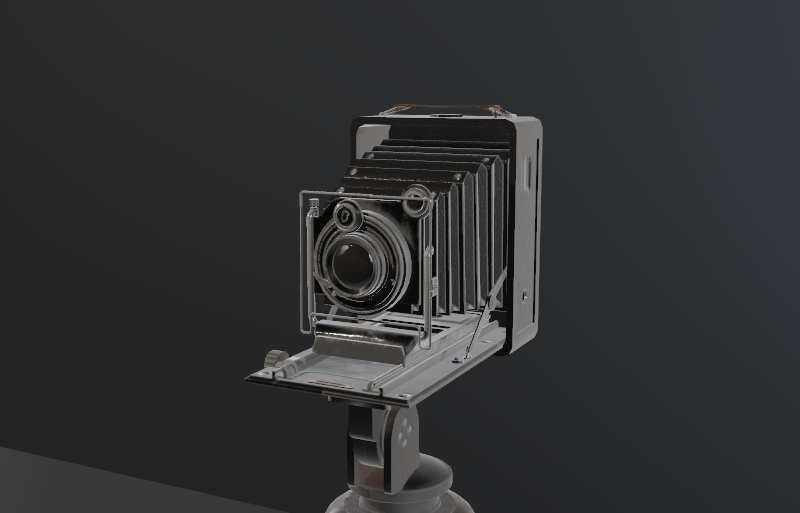
\includegraphics[width=.95\linewidth]{../../../output/profiling/material-studio/after.png}
\caption{正式 Vulkan 编辑器中的古董相机。机身使用模型自带的底色、法线和材质贴图，棚灯的倒影来自场景选定的 HDR 全景。}
\end{figure}

点开视口的\ui{实时效果}，关闭\ui{镜面 IBL}，再打开。机身右边框跟着变暗、变亮，两盏场景灯一直开着。要单独调灯，可在层级面板选\ui{主灯}，到\ui{属性 → 点光源}调整强度和半径。半径决定这盏灯最远能照到哪里。

想换一间摄影棚，先用\ui{另存为}留下场景副本，再从菜单栏的\ui{环境贴图}选择另一张 HDR 全景，或打开之前保存的 \path{.rfibl} 文件。\ui{镜面 IBL}控制金属和涂漆表面的环境倒影。把“间接光”选成\ui{环境漫反射 IBL}，全景也会照亮木头和皮革。换回\ui{DDGI}，则用房间里墙面之间传来的光计算漫反射。按 \ui{Ctrl + S} 可以留下这次的环境选择和效果开关。
\clearpage
\section{灯牌的颜色与花纹}
在 Vulkan 编辑器打开 \path{assets/scenes/Light-Studio.redflag}，切到\ui{主相机 Game}。模型和贴图已经随项目附上。房间里只有左边的灯牌发光，白墙和地板靠它照亮。灯牌的三条色带共用一份材质。上、下两条在贴图里是白色，中间一条是灰色，因此中间看起来暗一些。

\begin{figure}[H]\centering
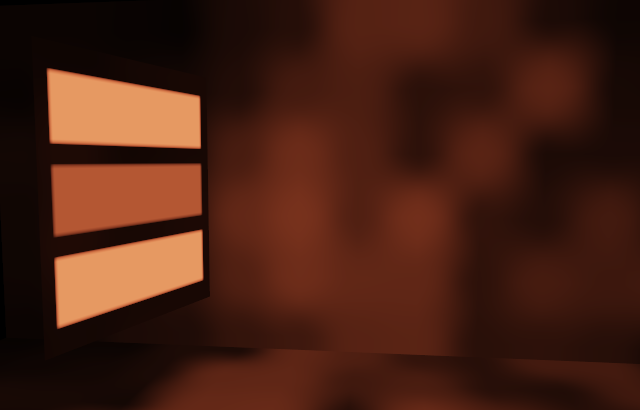
\includegraphics[width=.86\linewidth]{../../../output/profiling/emissive-studio/baked.png}
\caption{编辑器打开随场景保存的光照后，第 24 帧的画面。先看灯牌黑色边框和亮条的分界，再看右侧白墙：墙上能看见暖色，灯条的形状已经分辨不出来了。}
\end{figure}

在层级面板选中\ui{灯牌}，展开属性中的模型材质，勾选\ui{为此物体调整材质}。找到该部件的\ui{自发光}，其中三个数依次是红、绿、蓝。把红色调低，亮条和照在墙上的光都会变色。把三个数都设为零，房间会暗下来。若要改条纹，点\ui{选择自发光贴图}。白色区域发出材质设定的光，黑色区域熄灭。移除贴图后，整块面板都按同一种颜色发光。

要单看墙，切到\ui{场景 Scene}，移动镜头直到灯牌离开画面。在\ui{实时效果}里将间接光选为\ui{DDGI}，墙上仍能看到暖光。DDGI 在房间中许多固定位置计算光照，因此转动镜头时还知道灯牌在哪里。选好灯光后，到“质量与参数”点“烘焙探针”，再保存场景。再次改动灯牌的颜色、图片或位置时，需要重新烘焙才能把新光照留到下次打开。
\clearpage
\section{镜面与屏幕外反射}
打开 \path{assets/scenes/Mirror-Studio.redflag}，切到\ui{主相机 Game}。墙上的镜子正对着一块橙色灯牌。灯牌在相机身后，镜子里可以看清它的黑框、两条亮带和中间稍暗的一条。这个场景已经打开 SSR 和屏幕外反射，房间的光照也已烘焙好。

\begin{figure}[H]\centering
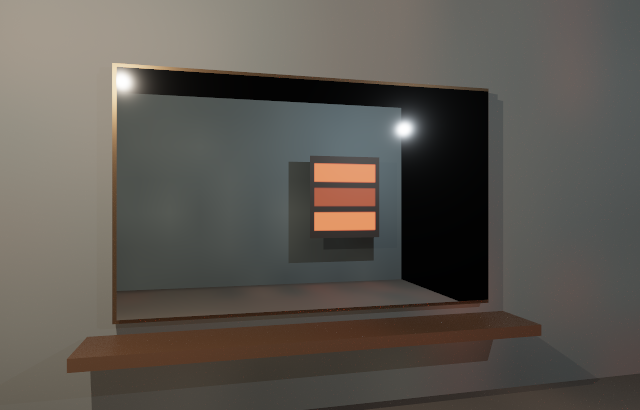
\includegraphics[width=.69\linewidth]{../../../output/profiling/scene-reflections/mirror-scene.png}
\caption{镜面工作室的场景面板。左右两点白色高光来自房间的点光源，中间的橙色条纹来自模型上的发光贴图。}
\end{figure}

展开场景面板的\ui{实时效果}。保持\ui{SSR}开启，只取消它下方的\ui{屏幕外反射}，灯牌的条纹就会消失。重新勾选，镜子又能照见身后的灯牌。在层级中选\ui{镜面}，拖动材质里的 \ui{Roughness}（粗糙度）。零对应光滑的镜面，调高后灯条边缘逐渐散开。

\noindent\shots{../../../output/profiling/scene-reflections/mirror-screen.png}{只开 SSR。相机看不到灯牌，镜中也找不到它。}\hfill
\shots{../../../output/profiling/scene-reflections/mirror-blocked.png}{打开屏幕外反射，在镜子与灯牌之间放一块板，镜中就出现板的颜色。}

要自己试遮挡，可用\ui{场景对象 → 立方体}创建挡板，将位置设为 $(1.07,1.53,2.55)$，缩放设为 $(1.12,1.28,0.12)$。沿水平方向移走它，灯牌会从挡板后面露出。想留下这一版布置，可先另存场景，再烘焙探针。
\clearpage
\section{浴室里的反射降噪}
打开 \path{assets/scenes/RTXGI-Bathroom.redflag}，切到\ui{主相机 Game}。在视口上方打开\ui{实时效果}，勾选 \ui{SSR}，看右手边窗框下的灰墙。浴室已选好\ui{屏幕外反射}和\ui{反射降噪}，打开 SSR 时这两项一起生效。这样即使物体在相机画面以外，也有机会出现在砖墙的倒影里。

\begin{figure}[H]\centering
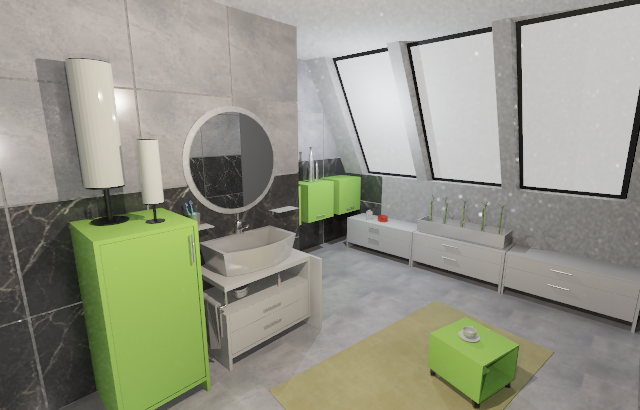
\includegraphics[width=.70\linewidth]{../../../output/profiling/rough-reflections/small-on.png}
\caption{浴室的主相机画面。下方的两张近照截取自右侧窗户、墙砖和洗手台所在的位置。}
\end{figure}

先关闭 \ui{TAA}，让面板只显示当前帧的颜色，再切换\ui{反射降噪}。左图的墙砖上散着许多亮点。开启降噪后，程序会参考同一块墙面上邻近像素的倒影。墙上的亮点减少了，深色窗框的位置仍看得清。停在右图仔细看，墙上还能见到小片的明暗差别。

\noindent\shots{../../../output/profiling/rough-reflections/detail-off.png}{关闭反射降噪。窗下的灰墙上散布着细小的亮点。}\hfill
\shots{../../../output/profiling/rough-reflections/detail-on.png}{开启反射降噪。两图取自同一机位、第 24 帧，均显示 TAA 混合颜色前的结果。}

比较完再打开 \ui{TAA}，让多帧的颜色一起改善窗框边缘。选“文件 → 另存为”可将这组开关保存在场景副本里。
\clearpage
\section{细线和斜边的取样}\label{sec:ssaa}
在 Vulkan 编辑器打开 Sponza 中庭。右下角是\ui{渲染设置}，将\ui{显示模式}设为\ui{组合光照 Lit}。先在\ui{实时效果}里关闭 TAA，再展开\ui{质量与参数}。将\ui{分辨率}设为 320，在同一机位勾选、取消\ui{SSAA 2×2}，看蓝布下方与黑色背景交界的拱线。

\begin{figure}[H]\centering
\begin{minipage}[c]{.55\linewidth}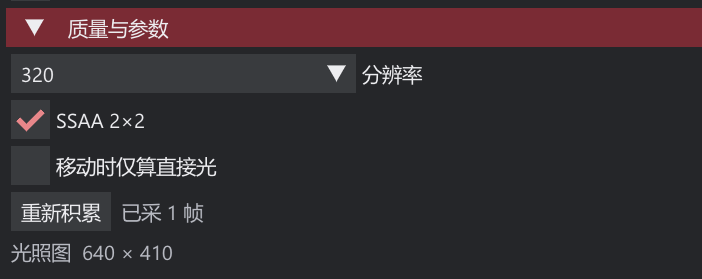
\includegraphics[width=\linewidth]{ssaa-settings.png}\end{minipage}\hfill
\begin{minipage}[c]{.39\linewidth}\caption{实际编辑器的“质量与参数”。面板输出选了 320 像素宽，开启 SSAA 后，内部计算光照的图宽 640 像素。}\end{minipage}
\end{figure}

\noindent\begin{minipage}[t]{.46\linewidth}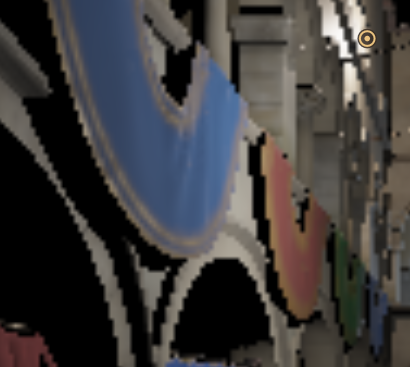
\includegraphics[width=\linewidth]{ssaa-sponza-off.png}\captionline{关闭。留意从蓝布下方向左上延伸的细线，以及拱线轮廓上的台阶。}\end{minipage}\hfill
\begin{minipage}[t]{.46\linewidth}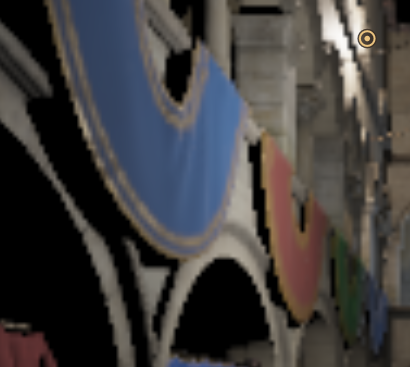
\includegraphics[width=\linewidth]{ssaa-sponza-on.png}\captionline{开启。两图截自同一机位的场景面板。内部光照图从 $320\times205$ 变为 $640\times410$。}\end{minipage}

这里的 $2\times2$ 表示把一个画面像素分成横向两格、纵向两格。若其中一格看见栏杆，另三格看见石墙，场景面板就会同时显示一点栏杆的颜色和更多的石墙颜色。SSAA 在一帧里完成这四次取样。重新打开 TAA 后，画面还会利用以前几帧的颜色。

\ui{SSAA 2×2} 默认关闭。如果界面提示降低分辨率，先在上方选较小的宽度。点击物体时，编辑器用单独的一张图查询鼠标位置的实体编号。像素边上带了一点铁丝颜色，仍有可能点到后面的墙。

按 \ui{Ctrl + S} 保存开关。想留下练习副本，可用\ui{文件 → 另存为}。
\end{document}
